\section{Traceroute}

\subsection{Traceroute, -N 20/30/40 vs Default}
Osservando i valori della detection si vede come questi siano esattamente identici (68 microsecondi) per i tre esperimenti con l'opzione -N, mentre sia leggermente più bassa (42 microsecondi) per quanto riguarda l'attacco traceroute di default. Rispetto alla durata dell'attacco, come ci si aspetta questa aumenta all'aumentare del numero di pacchetti-sonda inviati dal comando, mentre rimane circa a metà strada tra -N 30 e -N 40 per quanto riguarda la versione standard di traceroute. Quindi, dal momento che il manuale afferma che il valore di default per i pacchetti-sonda è 16, dai valori di durata della versione standard possiamo supporre che quest'ultima esegua operazioni in più, o più complesse, rispetto al comando che utilizza l'opzione -N.\\

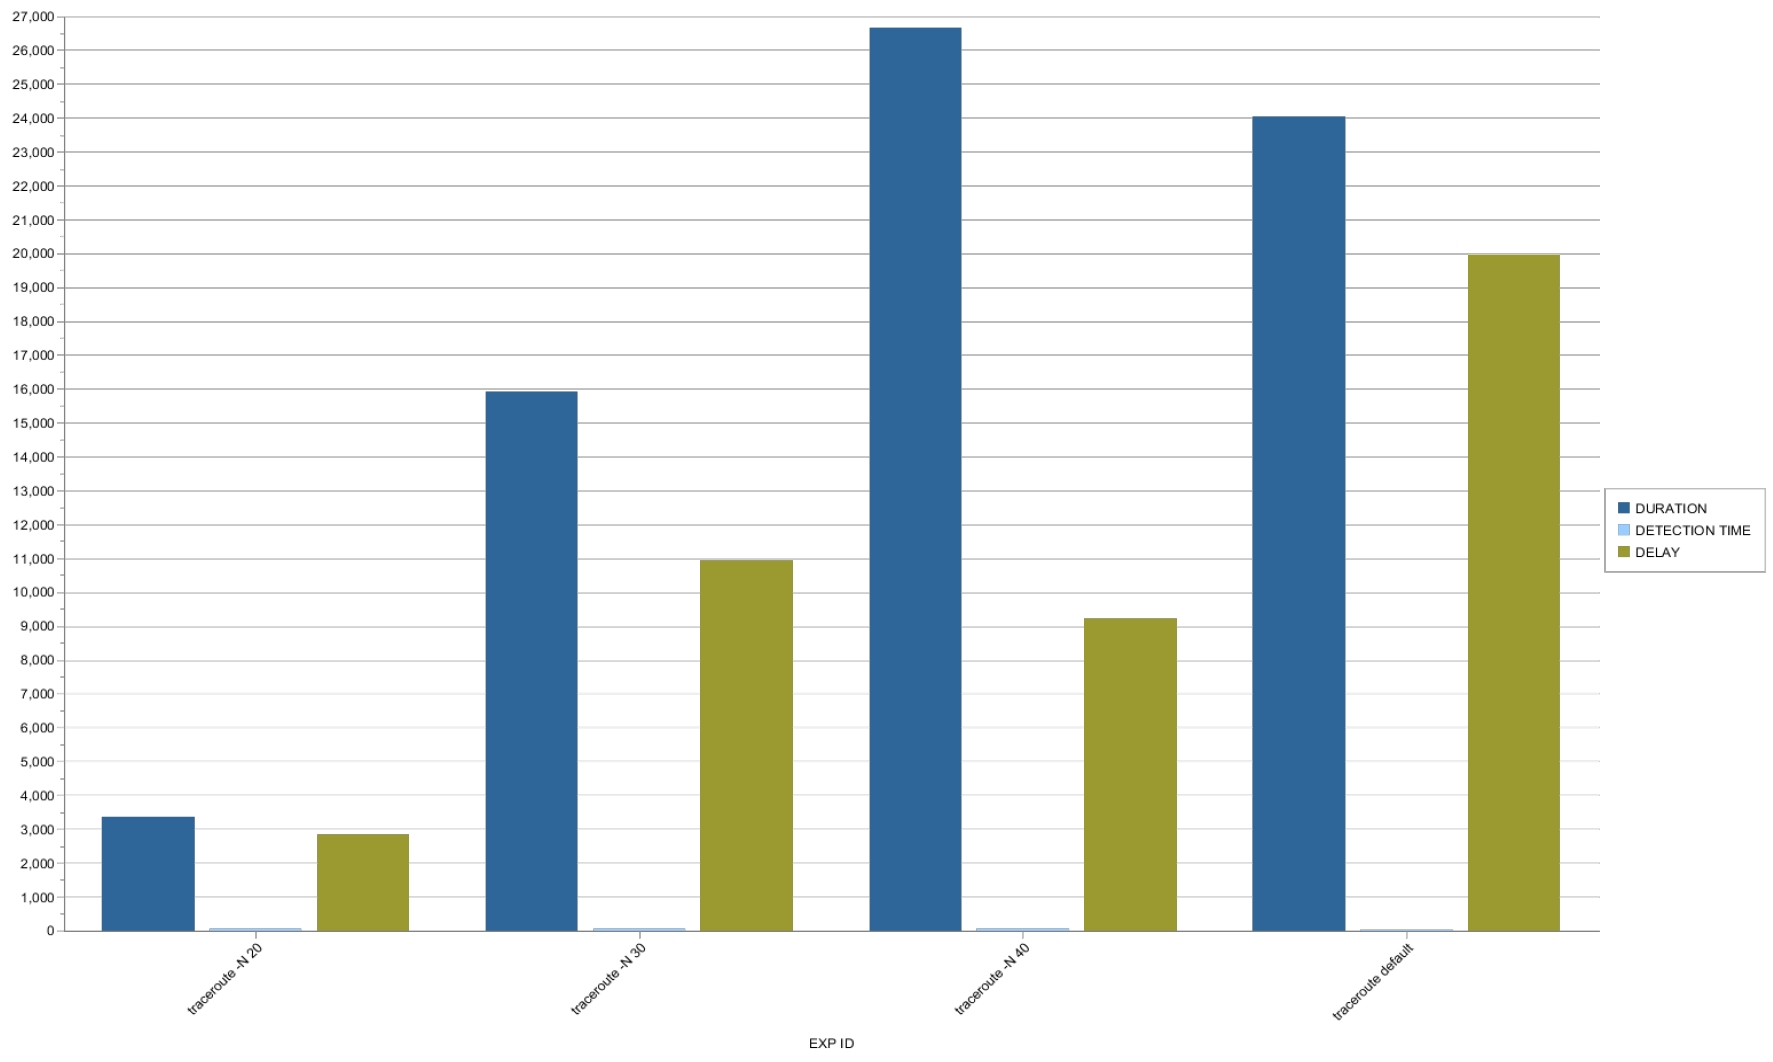
\includegraphics[scale=0.3]{figure/tempi_traceroute_N.jpg}\\

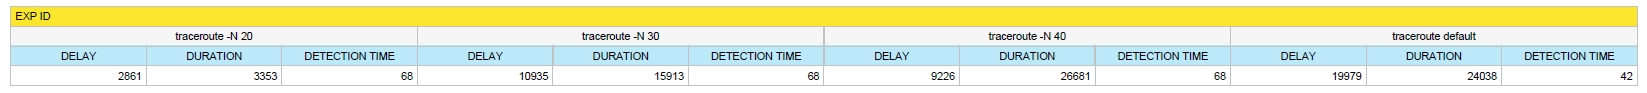
\includegraphics[scale=0.3]{figure/tabella_traceroute_N.jpg}

\subsection{Traceroute, -T vs Default}
In questi grafici, per comodità, sono stati omessi i valori di detection in quanto, come già accennato, il comando traceroute con opzione -T non genera alcun alert da parte di Snort. Si è comunque deciso di includere gli altri valori in quanto, dalla parte del sistema attaccato, vengono comunque ricevuti e loggati molti pacchetti che evidenziano, ad esempio, la maggior complessità dell'attacco traceroute -T, che impiega più tempo a terminare la scansione rispetto alla versione standard di traceroute.\\

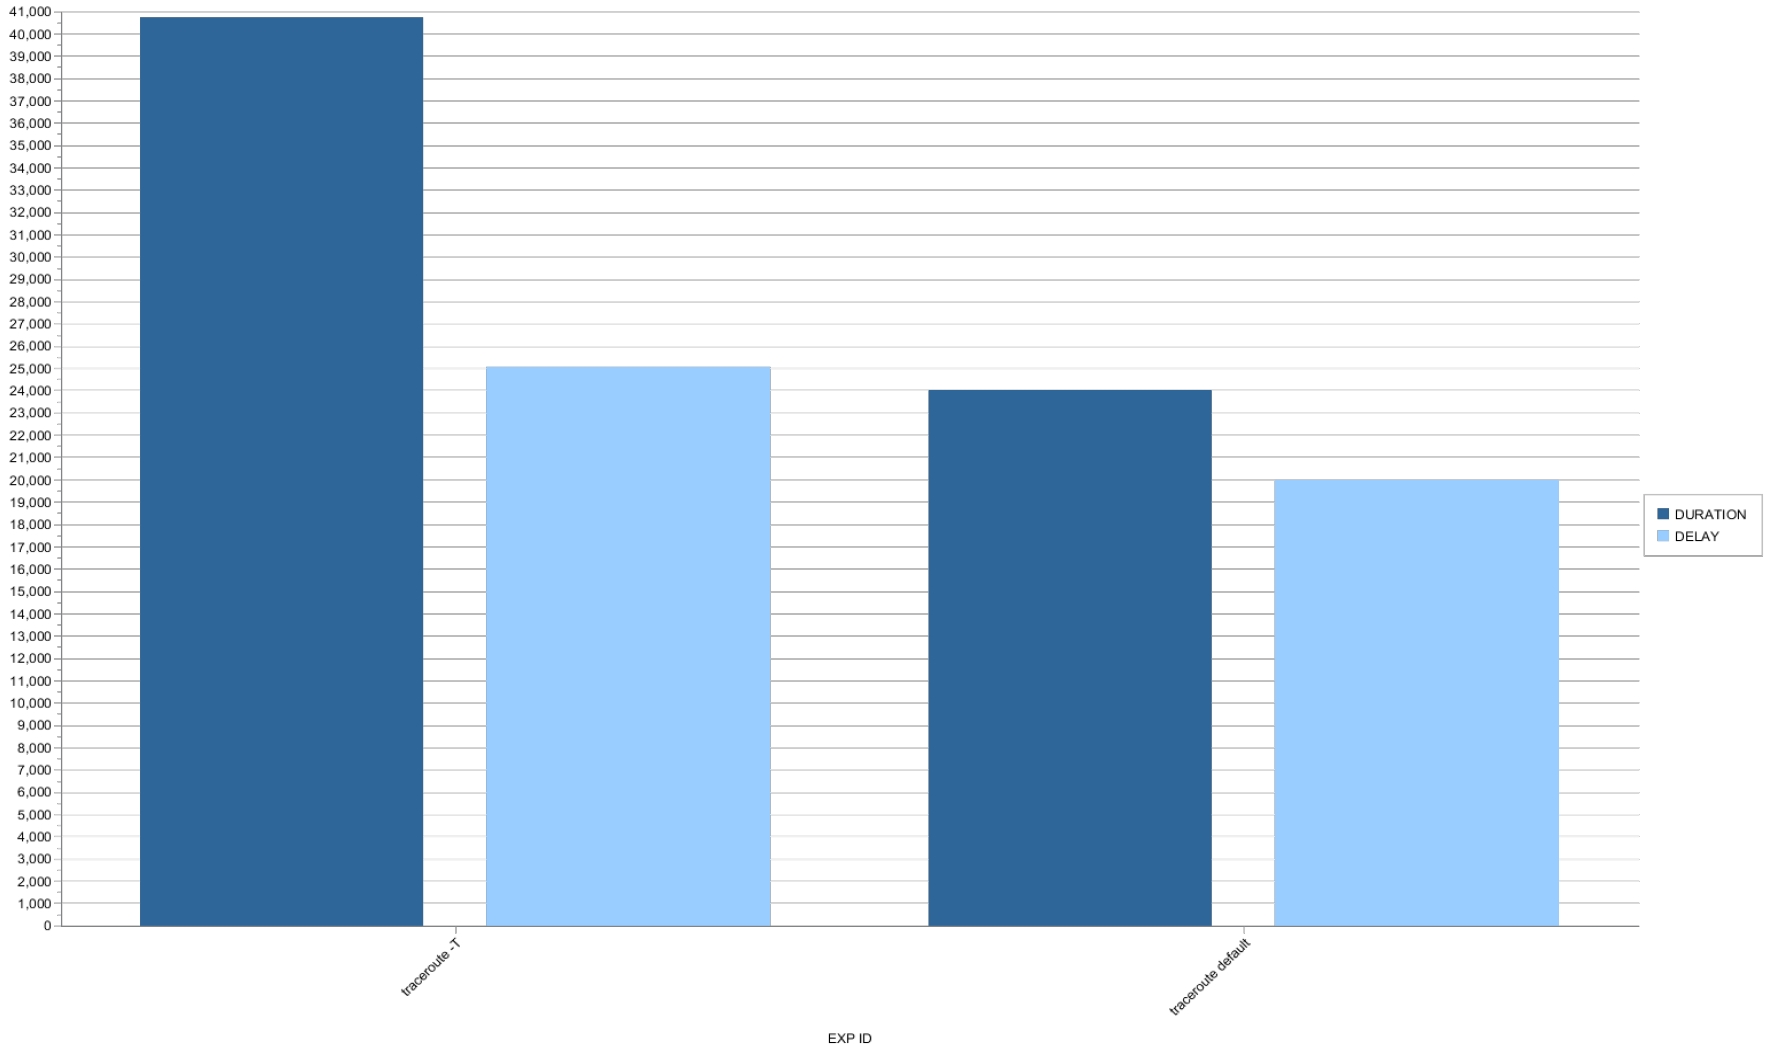
\includegraphics[scale=0.3]{figure/tempi_traceroute_T.jpg}\\

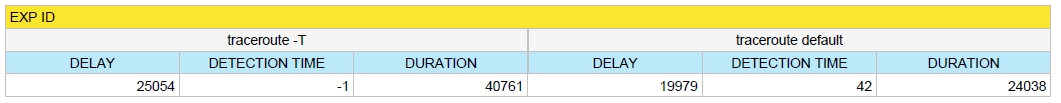
\includegraphics[scale=0.3]{figure/tabella_traceroute_T.jpg}

\subsection{Traceroute -I vs Default}
Come ci potevamo attendere, indicando a traceroute di eseguire un attacco tramite pacchetti ICMP ECHO si avrà che quest'attacco verrà identificato immediatamente (ovvero all'arrivo del primo pacchetto) da parte di Snort sul sistema attaccato. Infatti sappiamo che qualsiasi ping ricevuto da Snort verrà immediatamente loggato come alert. A parte questo, notiamo come (analogamente a quanto visto per l'opzione -T) la durata complessiva dell'attacco sia maggiore includendo l'opzione -I, che probabilmente aggiunge complessità all'attacco base di traceroute.\\

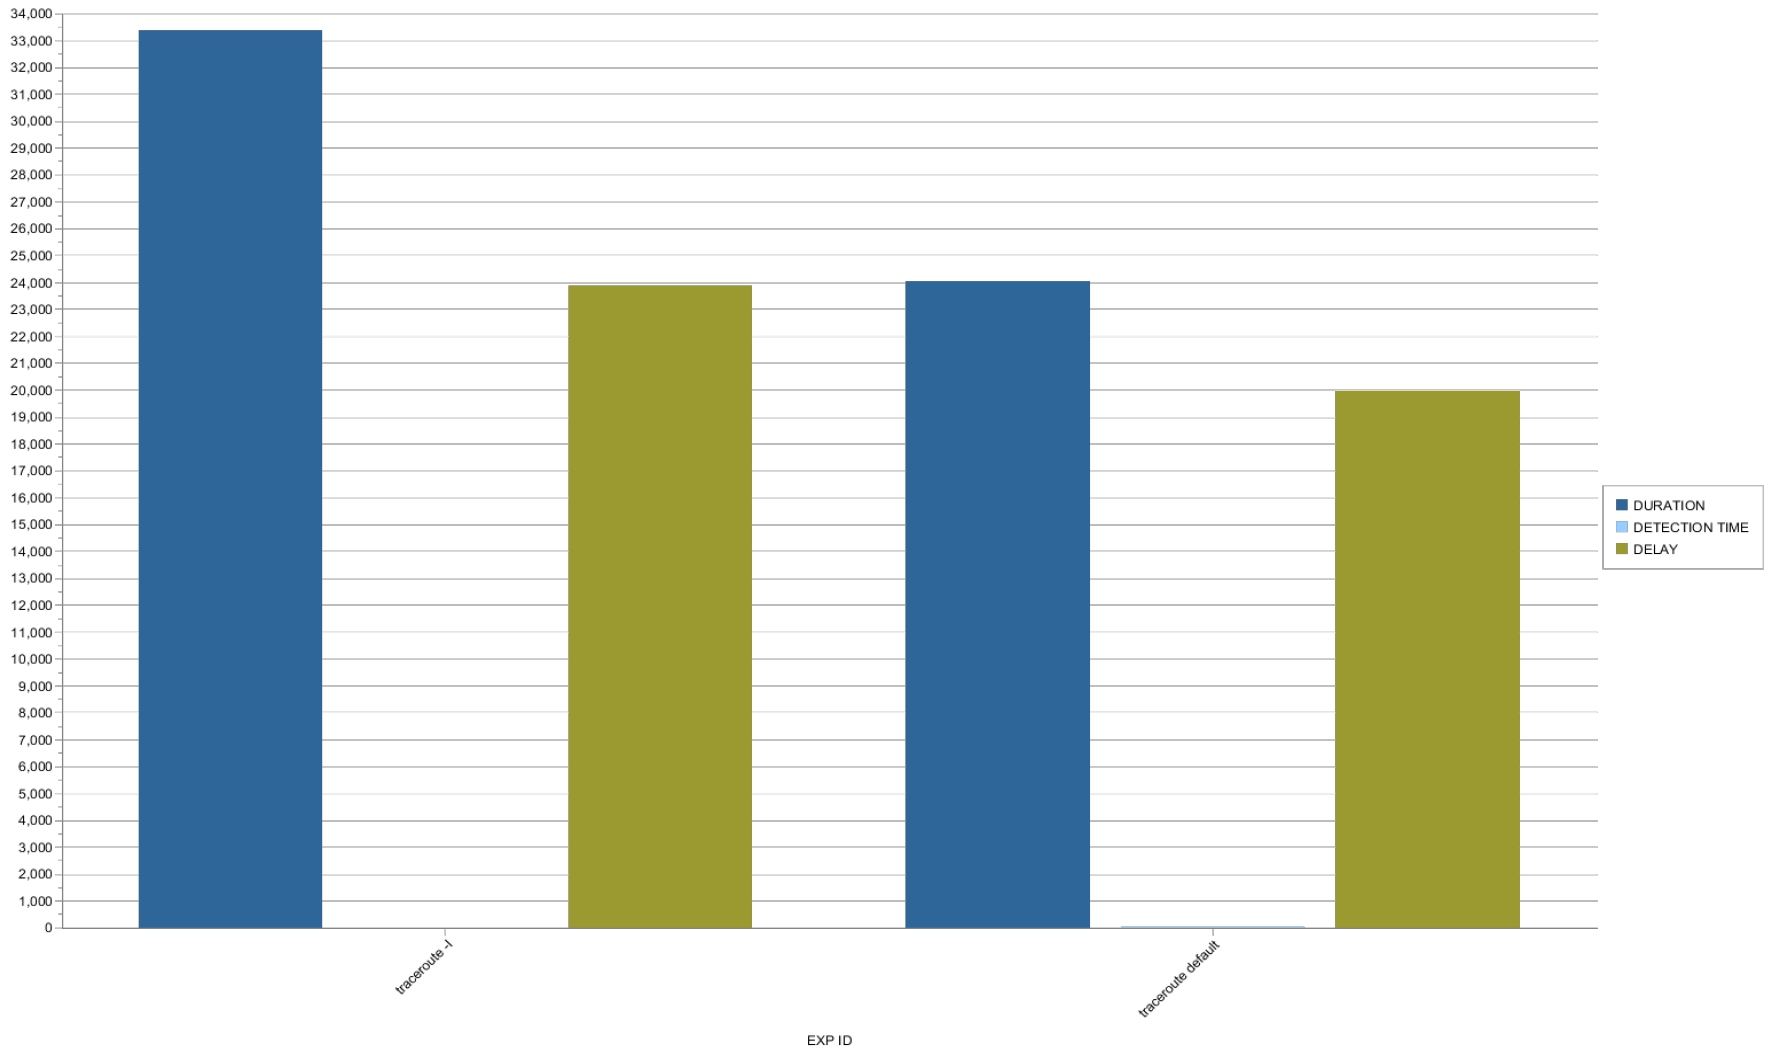
\includegraphics[scale=0.3]{figure/tempi_traceroute_I.jpg}\\

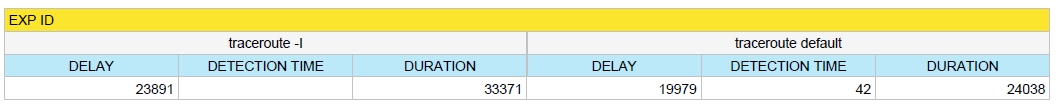
\includegraphics[scale=0.3]{figure/tabella_traceroute_I.jpg}
